\documentclass[journal]{vgtc}                % final (journal style)
%\documentclass[review,journal]{vgtc}         % review (journal style)
%\documentclass[widereview]{vgtc}             % wide-spaced review
%\documentclass[preprint,journal]{vgtc}       % preprint (journal style)

%% Uncomment one of the lines above depending on where your paper is
%% in the conference process. ``review'' and ``widereview'' are for review
%% submission, ``preprint'' is for pre-publication, and the final version
%% doesn't use a specific qualifier.

%% Please use one of the ``review'' options in combination with the
%% assigned online id (see below) ONLY if your paper uses a double blind
%% review process. Some conferences, like IEEE Vis and InfoVis, have NOT
%% in the past.

%% Please use the ``preprint''  option when producing a preprint version
%% for sharing your article on an open access repository

%% Please note that the use of figures other than the optional teaser is not permitted on the first page
%% of the journal version.  Figures should begin on the second page and be
%% in CMYK or Grey scale format, otherwise, colour shifting may occur
%% during the printing process.  Papers submitted with figures other than the optional teaser on the
%% first page will be refused. Also, the teaser figure should only have the
%% width of the abstract as the template enforces it.

%% These few lines make a distinction between latex and pdflatex calls and they
%% bring in essential packages for graphics and font handling.
%% Note that due to the \DeclareGraphicsExtensions{} call it is no longer necessary
%% to provide the the path and extension of a graphics file:
%% 
\includegraphics{diamondrule} is completely sufficient.
%%
\ifpdf%                                % if we use pdflatex
  \pdfoutput=1\relax                   % create PDFs from pdfLaTeX
  \pdfcompresslevel=9                  % PDF Compression
  \pdfoptionpdfminorversion=7          % create PDF 1.7
  \ExecuteOptions{pdftex}
  \usepackage{graphicx}                % allow us to embed graphics files
  \DeclareGraphicsExtensions{.pdf,.png,.jpg,.jpeg} % for pdflatex we expect .pdf, .png, or .jpg files
\else%                                 % else we use pure latex
  \ExecuteOptions{dvips}
  \usepackage{graphicx}                % allow us to embed graphics files
  \DeclareGraphicsExtensions{.eps}     % for pure latex we expect eps files
\fi%

%% it is recomended to use ``\autoref{sec:bla}'' instead of ``Fig.~\ref{sec:bla}''
\graphicspath{{figures/}{pictures/}{images/}{./}} % where to search for the images

\usepackage{microtype}                 % use micro-typography (slightly more compact, better to read)
\PassOptionsToPackage{warn}{textcomp}  % to address font issues with \textrightarrow
\usepackage{textcomp}                  % use better special symbols
\usepackage{mathptmx}                  % use matching math font
\usepackage{times}                     % we use Times as the main font
\renewcommand*\ttdefault{txtt}         % a nicer typewriter font
\usepackage{cite}                      % needed to automatically sort the references
\usepackage{tabu}                      % only used for the table example
\usepackage{booktabs}                  % only used for the table example
\usepackage[shortlabels]{enumitem}                  % for ordered lists with a/b/c
%% We encourage the use of mathptmx for consistent usage of times font
%% throughout the proceedings. However, if you encounter conflicts
%% with other math-related packages, you may want to disable it.

%% In preprint mode you may define your own headline. If not, the default IEEE copyright message will appear in preprint mode.
%\preprinttext{To appear in IEEE Transactions on Visualization and Computer Graphics.}

%% In preprint mode, this adds a link to the version of the paper on IEEEXplore
%% Uncomment this line when you produce a preprint version of the article 
%% after the article receives a DOI for the paper from IEEE
%\ieeedoi{xx.xxxx/TVCG.201x.xxxxxxx}

%% If you are submitting a paper to a conference for review with a double
%% blind reviewing process, please replace the value ``0'' below with your
%% OnlineID. Otherwise, you may safely leave it at ``0''.
\onlineid{0}

%% declare the category of your paper, only shown in review mode
%%\vgtccategory{Research}
%% please declare the paper type of your paper to help reviewers, only shown in review mode
%% choices:
%% * algorithm/technique
%% * application/design study
%% * evaluation
%% * system
%% * theory/model
%%\vgtcpapertype{please specify}

%% Paper title.
\title{Pandemic Pedagogy: Taking Data-Viz Learning Online}

%% This is how authors are specified in the journal style

%% indicate IEEE Member or Student Member in form indicated below
\author{Rahul Bhargava}
\authorfooter{
%% insert punctuation at end of each item
\item
 Rahul Bhargava is with the Northeastern School of Journalism. E-mail: r.bhargava@northeastern.edu.
}

%other entries to be set up for journal
\shortauthortitle{Bhargava: Pandemic Pedagogy}
%\shortauthortitle{Firstauthor \MakeLowercase{\textit{et al.}}: Paper Title}

%% Abstract section.
%%\abstract{Duis autem vel eum iriure dolor in hendrerit in vulputate
%%} % end of abstract

%% Keywords that describe your work. Will show as 'Index Terms' in journal
%% please capitalize first letter and insert punctuation after last keyword
%%\keywords{Radiosity, global illumination, constant time}

%% ACM Computing Classification System (CCS). 
%% See <http://www.acm.org/class/1998/> for details.
%% The ``\CCScat'' command takes four arguments.

%%\CCScatlist{ % not used in journal version
%% \CCScat{K.6.1}{Management of Computing and Information Systems}%
%%{Project and People Management}{Life Cycle};
%% \CCScat{K.7.m}{The Computing Profession}{Miscellaneous}{Ethics}
%%}

%% A teaser figure can be included as follows
%%\teaser{
%%  \centering
%%  \includegraphics[width=\linewidth]{CypressView}
%%  \caption{In the Clouds: Vancouver from Cypress Mountain. Note that the teaser may not be wider than the abstract block.}
%%  \label{fig:teaser}
%%}

%% Uncomment below to disable the manuscript note
\renewcommand{\manuscriptnotetxt}{}

%% Copyright space is enabled by default as required by guidelines.
%% It is disabled by the 'review' option or via the following command:
% \nocopyrightspace


\vgtcinsertpkg

%%%%%%%%%%%%%%%%%%%%%%%%%%%%%%%%%%%%%%%%%%%%%%%%%%%%%%%%%%%%%%%%
%%%%%%%%%%%%%%%%%%%%%% START OF THE PAPER %%%%%%%%%%%%%%%%%%%%%%
%%%%%%%%%%%%%%%%%%%%%%%%%%%%%%%%%%%%%%%%%%%%%%%%%%%%%%%%%%%%%%%%%

\begin{document}

%% The ``\maketitle'' command must be the first command after the
%% ``\begin{document}'' command. It prepares and prints the title block.

%% the only exception to this rule is the \firstsection command
\firstsection{Introduction}

\maketitle

%% \section{Introduction} %for journal use above \firstsection{..} instead
Data visualization has become firmly established as a critical and increasingly mainstream communication technique for our data-centered times. It is being taught in multiple fields - from journalism\cite{gray_data_2012}, to undergraduate computer science education\cite{syeda_design_2020}, to business schools\cite{wolfe_teaching_2015} and more. In both \href{https://vgl.cs.usfca.edu/pdvw/2016/}{2016} and \href{https://vgl.cs.usfca.edu/pdvw/2017/}{2017} this conference hosted workshops on the "Pedagogy of Data Visualization".

In the midst of a global pandemic, how do we continue to deliver creative and high-quality learning experiences for data visualization online? This short paper introduces two case studies of how I have taken hands-on activities related to data visualization and brought them online. They demonstrate to me that when considering moving an activity online one should ask themselves questions such as:
\begin{enumerate}
  \itemsep0em 
  \item Can the activity be moved online without sacrificing learning goals and pedagogy?
  \item What parts of the activity might your technology support? What parts might it hinder?
  \item How can you turn the students’ physical space limitations into an opportunity?
\end{enumerate}
I don’t consider these to be radically new questions in the world of online  teaching. I reiterate them here, in the time of a global pandemic, to reinforce that simply moving activities online as-is is unlikely to produce strong learning outcomes.

\section{Motivation}
My approach to data visualization education is firmly rooted in principles of hands-on learning and constructionism\cite{dignazio_creative_2018}. I anchor my pedagogy in this central idea of Seymour Papert’s – that learning occurs best when people are designing and discussing objects for audiences that are meaningful to themselves or their peers\cite{papert_childrens_1994}. As businesses and campuses emptied and teaching moved online, I quickly began to reflect on what it meant to create constructionist experiences for data visualization learning in virtual settings.

Our \href{https://datacultureproject.org}{Data Culture Project} already offers a  set of participatory, hands-on activities for learning various stages of the data visualization process. The dozen activities documented there function as a self-service curriculum online, used by tens of thousands across the globe to support learning in educational, non-profit, and business settings. 

During the spring 2020 disruption I adapted and used two of the Data Culture Project activities in virtual classroom settings, as documented in the following sections. Each example pulls from my experiences this past spring taking my small undergraduate/graduate university “Data Storytelling Studio” course online due to the pandemic. The class included 18 students, meeting co-temporally in a Zoom room twice a week for roughly a third of the spring semester. Students came from various disciplines - business, education, public health, urban planning, engineering, computer science.

\section{Case Study 1: Building Data Sculptures}
The “Build a Data Sculpture” activity invites participants to build a physical representation of a data story using familiar craft materials within 10 minutes. In prior work I argue that this activity is particularly well-suited to environments that benefit from a low-tech and playful introduction to working with data \cite{bhargava_data_2017}. As part of a semester long course, I've previously expanded this to be a 2-week group project.

Rescheduling caused by the pandemic made that impossible. I ran through a few options for taking this online which considering the three guiding questions I opened with:
\begin{enumerate}[(a)] % (a), (b), (c), ...
  \itemsep0em 
  \item Eliminate it from my syllabus
  \item Have students remotely collaborate while one builds
  \item Have students build with their own materials at home
  \item Mail students a standard box of materials to build with
\end{enumerate}

\begin{figure}[h]
  \centering
  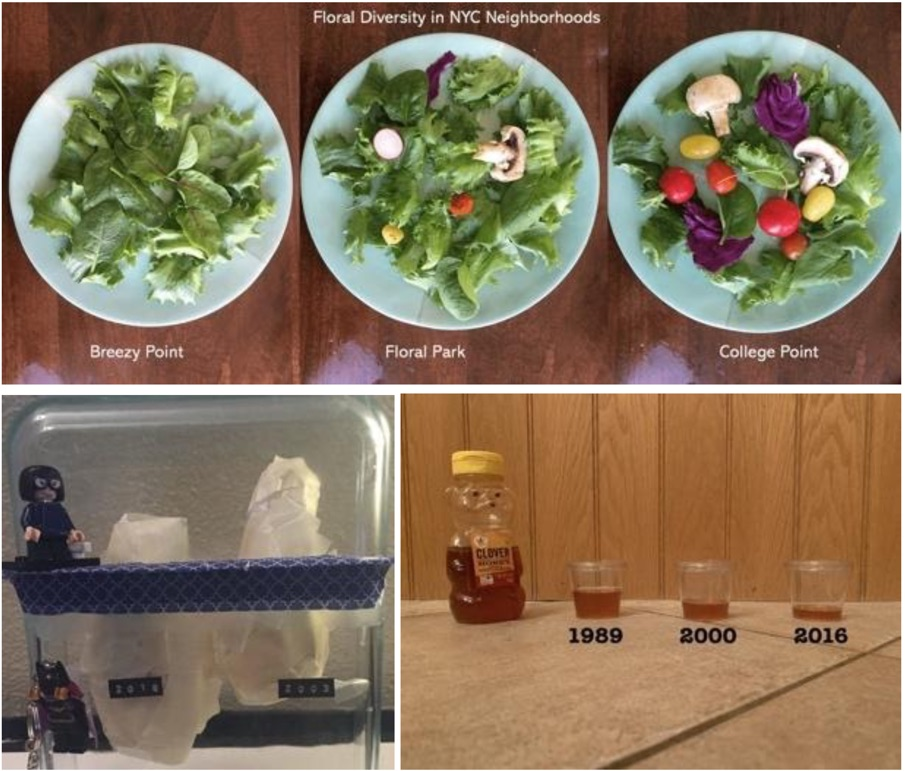
\includegraphics[scale=0.26]{figures/figure1.jpg}
  \label{fig:data_sculpture_examples}
  \caption{Data sculptures created by students.}
\end{figure}

After weighing the various affordances, I decided to have them build small data sculptures individually with whatever they found around them (c). This maintained my learning goals and pedagogy, because it still offered them a chance to play with physical information encodings. I asked them to post photos of their projects to the class blog, in order to allow the creation process to avoid any technological intermediation but also support sharing and discussion.  To connect the assignment to their interests, I asked them to work with a data story they had already created in one of the two previous group projects they had worked on. I felt this would focus the activity on the material affordances and evocative power of the physical objects they use, rather than on the story-finding process. This approach also turned their physical constraints into a positive, because they each would have different materials around them and would likely produce a diversity of approaches and projects.

The students built  data sculptures that showed far more creativity than when I run the activity in the standard way (see Fig. 1). One used the amount of salad toppings to indicate floral diversity in different parts of New York City. Another smudged a globe with dirty fingerprints to encode air pollution. A third built a model of a two-storey museum exhibit that portrayed accepted vs. denied US FOIA requests with a "tip of the iceberg" metaphor. As a whole, the sculptures captured each of Moere and Patel's "symbolic, iconic and indexical" taxonomy\cite{moere_physical_2009}. These results lead me to believe that this approach to taking the data sculptures activity online met my criteria for success quite well; my plan responded well enough to my three guiding questions to produce evocative projects that provoked discussion.

\section{Case Study 2: Sketching a Visual Word Web}
The "word webs" activity is used by artists to help move a group from an abstract concept to a larger set of words that describe it. In the data visualization process this can help transition from abstract concepts such as “power”, “justice”, or “community“ to more easily depicted terms such as "hammer", "scale", or "holding hands". As part of my Data Murals process I adapt this technique to create collaborative pictographic word webs, helping brainstorm a symbol language for a data story\cite{bhargava_data_2016}.

\begin{figure}[h]
  \centering
  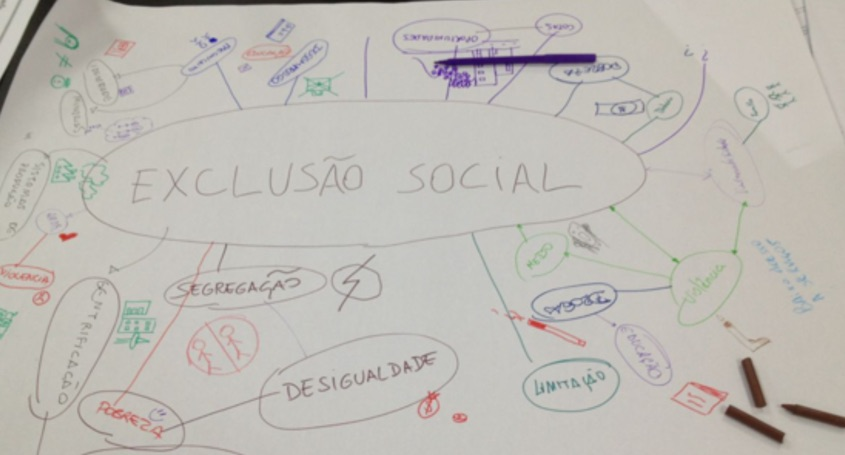
\includegraphics[scale=0.26]{figures/figure2.jpg}
  \label{fig:full_word_web}
  \caption{A pictographic word web created in person to tease out a symbolic language for “social exclusion” (in Brazilian Portuguese).}
\end{figure}

The activity begins with a large piece of paper with the central word of the story written on it. Each learner brainstorms connected words, in silence, and writes them on the paper, connecting each new word to the word that inspired it with a line. After about 5 minutes we hand out post-it notes and ask the participants to look for ideas that are easy to illustrate, draw each one on an individual sticky note, and stick it near the word that it illustrates (see an example in Fig. 2).

Rethinking this activity for a virtual setting, I found some tradeoffs needed to be made. I could support the participatory nature of it by using the virtual whiteboard feature built into our Zoom meeting. I found most students familiar with the technology from other classes they were in that had already used it. It allowed for collaborative writing to happen with real-time synchronization, so everyone could see what the other students were writing. Unfortunately the joy of moving around a large paper, leaning in and stepping back, didn't feel like it would translate well to this technology. The serendipity of moving around the table lends a lot to this activity, so I was unsure of success.

I found that the first phase of word generation worked well, but the sketching process fell flat. The group of students created a word web that I qualitatively assessed to be similar in variety of scope to those made in physical settings (see Fig. 3).  However, when we tried to shift into the sketching portion of the activity it fell apart. Students found it hard to sketch with the virtual tools provided, expressing frustration with pixelated drawings “not coming out the way I wanted”, wondering “where should I draw?”, and laughing at what they had drawn. As those frustrations mounted I decided to end the activity early. 

\begin{figure}[h]
  \centering
  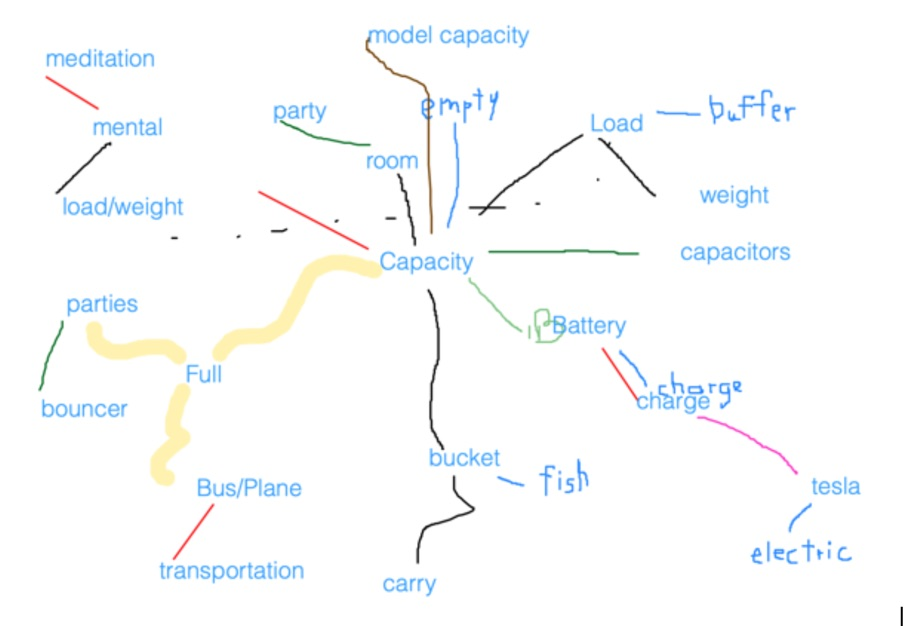
\includegraphics[scale=0.26]{figures/figure3.jpg}
  \label{fig:online_word_web}
  \caption{A collaborative word web created in a Zoom online class using the built-in whiteboard. The central word was “capacity”.}
\end{figure}

In reflection, I attribute this to the affordances of the particular technology I chose - it both supported and hindered the activity. It didn't allow for detailed sketching. That isn’t a criticism of the tool so much as a recognition of its intent. Sketching in a virtual environment, even with the goal of stick-figure like cartoon drawings, requires a different UI design and I, as the teacher, shouldn’t have assumed Zoom’s whiteboard would accommodate both interaction needs. In addition, I ignored the third of my guiding questions - I didn't turn the student's physical constraints into a positive. Another approach could be to have students draw sketches on sticky notes and post photos to an image board (using Pinterest or some other similar tool). On the whole this activity presented more challenges to being run virtually while still fully addressing my three guiding questions.


\section{Conclusion}
The coronavirus pandemic seems certain to snarl fall teaching plans, requiring many data visualization learning environments to stay online. We hope these two examples of translating hands-on participatory data visualization learning activities to the virtual setting are valuable to workshop participants. Intentionally designing virtual participatory data visualization learning activities requires us as educators to constantly revisit our guiding principles. I have shared an initial three in this article and discussed how they informed my process - retaining pedagogy and learning goals, carefully considering technological affordances, and taking advantage of student's physical constraints.

%% if specified like this the section will be committed in review mode
\acknowledgments{
I'd like to thank artist Tova Speter for introducing me to the word web activity, Emily Bhargava and  Catherine D'Ignazio for comments, and my students for surviving the ups and downs of a turbulent semester.
}

%\bibliographystyle{abbrv}
\bibliographystyle{abbrv-doi}
%\bibliographystyle{abbrv-doi-narrow}
%\bibliographystyle{abbrv-doi-hyperref}
%\bibliographystyle{abbrv-doi-hyperref-narrow}

\bibliography{template}
\end{document}

